\subsubsection{\stid{1.17} Open~MPI for Exascale (OMPI-X)}\label{subsubsect:openmpi}

%% {\itshape

%% 	\begin{enumerate}
%% 	\item Rename this file to your project WBS-projectname.tex, for example 2.3.3.01-XSDK4ECP.tex.
%% 	\item Complete this template for your project.  Limit your text to two pages, not counting citations.
%% 	\item Please avoid changing the content of main.tex.
%% 	\item Put any references in a .bib file with the same root name, for example 2.3.3.01-XSDK4ECP.bib.
%% 	\item Remember to include any image files you reference in your text.
%%     \item The files 2.3.3.01-XSDK4ECP.tex, 2.3.3.01-XSDK4ECP.bib and xSDK-diagram.jpeg are included as examples for your reference.  You can remove them from what you upload.
%% 	\end{enumerate}
%% }

\paragraph{Overview}
%% \textit{Provide an overview of your project.  You might find that the introductory text from your Fall 2017 Project Summary \url{https://confluence.exascaleproject.org/display/1ST/Fall+2017+ECP+ST+Project+Summaries} useful as a starting draft.}

The OMPI-X project ensures that the Message Passing Interface (MPI)
standard, and its specific implementation in Open~MPI meet the needs
of the ECP community in terms of performance, scalability, and
capabilities or features. MPI is the predominant interface for
inter-process communication in high-end computing.  Nearly all of the
ECP application (AD) projects (93\%~\cite{Bernholdt:2018:SMU-tr})
and the majority of ST projects
(57\%~\cite{Bernholdt:2018:SMU-tr}) rely on it.
With the impending exascale era, the
pace of change and growing diversity of HPC architectures pose new
challenges that the MPI standard must address.  The OMPI-X project is
active in the MPI Forum standards organization, and works within it to
raise and resolve key issues facing ECP applications and libraries.

Open~MPI is an open source, community-based implementation of the MPI
standard that is used by a number of prominent
HPC vendors as the basis for their commercial MPI offerings.   The
OMPI-X team is comprised of active members of the Open~MPI community,
with an extensive history of contributions to this community.
The OMPI-X project focuses on prototyping
and demonstrating exascale-relevant proposals under consideration by
the MPI Forum, as well as improving the fundamental performance and
scalability of Open~MPI, particularly for exascale-relevant platforms
and job sizes.
MPI users will be able to take advantage of these
enhancements simply by linking against recent builds of the Open~MPI
library.

In addition to MPI and Open~MPI, the project also includes two other products,
which are less visible to the end user, but no less important.
PMIx (Process Management Interface for Exascale) provides facilities for
scalable application launch, process wire-up, resilience, and coordination between runtimes.
It originated as a spin-off from the Open~MPI community, but is now developing a
community of its own as adoption grows.  Starting in FY20,
Qthreads (formerly WBS 2.3.1.15) is also part of the OMPI-X project.  Qthreads is a
user-level lightweight asynchronous thread library particularly focused on improving support for
multithreading in the context of network communications.  Both PMIx and Qthreads help the
OMPI-X project address key issues of performance and capability for exascale applications.


\paragraph{Key  Challenges}
%% \textit{Describe what is hard to do, why it is challenging.}
A number of aspects of ``exascale'' levels
of computing pose serious challenges to the ``tried and true'' message
passing model presented by MPI and its implementations, including Open~MPI.
%
Keeping pace with changes in HPC architecture is a major challenge.
Examples include massive node-level concurrency, driving the
growth of ``MPI+X'' programming approaches,
and the complex memory architectures, which make the placement of data
within memory more important. In the near-term, with GPUs dominating the exascale
environment, how code running on the GPUs interacts with MPI and inter-process
communications must also be addressed.  This will require both changes to the standard
and changes and improvements within implementations.
%
Performance and scalability become both more important and more
challenging as node counts increase
and memory per MPI rank trends downward.
%
Finally, as we identify solutions to these challenges that must be
``implemented'' within the MPI \emph{standard} rather than particular MPI libraries,
we must work within the much larger and broader MPI
community that may not always be attuned to the needs of computing at the largest scales.

\paragraph{Solution Strategy}
%% \textit{Describe your basic strategy for addressing the challenges.}
The OMPI-X project is working across a number of fronts to address
these challenges.

\emph{Runtime Interoperability for MPI+X and Beyond} MPI is
increasingly being used concurrently with other runtime environments.
This includes both ``MPI+X'' approaches, where X
is most often a threading model, such as OpenMP, as
well as the use of multiple inter-process runtimes within a single
application.  Concerns include awareness of other runtimes,
cooperative resource management capabilities, and ensuring that all
concurrently active runtimes make progress.  We are developing APIs and
demonstrating capabilities for interoperability in both MPI+X and
multiple inter-process runtime situations.

\emph{Extending the MPI Standard to Better Support Exascale
Architectures} The MPI community is standardizing a
number of ideas that
are particularly important to supporting
the architectural and system size characteristics anticipated for
exascale.  ``Partitioned communications'' (previously called ``Finepoints'')
deal with the growing use of threading for node-level concurrency, in
combination with MPI.  ``Sessions'' increases the flexibility of MPI
semantics in a number of areas, which in turn can open opportunities
for enhanced scalability, as well as easier support for
multi-component applications such as coupled multi-physics
simulations. Error management and recovery capabilities are key to
ensuring that applications can detect and respond effectively when errors,
inevitably, occur during execution.  We are helping to drive incorporation
of these and other ideas into the MPI standard by developing prototypes and
working with ECP teams and the broader community to demonstrate their
feasibility and value.

\emph{Open~MPI Scalability and Performance} As we push the scale of
both hardware and applications, we stress MPI implementations and
expose areas that need to be improved.
OMPI-X is targeting key components within Open~MPI, such as threading capabilities,
memory usage, remote memory access (RMA), tag matching, and other areas,
for improvements in both scalability and performance.

\emph{Supporting More Dynamic Execution Environments} We are
developing and implementing strategies to help MPI applications
better deal with topological process layout preferences
and contention in the network.

\emph{Resilience in MPI and Open~MPI} Concerns about system and
application resilience increase as either scales in size.  Our goal in
this area is to ensure that MPI, Open~MPI, and PMIx provide not only
support for simplified
recovery for the widely used checkpoint/restart fault tolerance strategy, but also the building
blocks to support more general error management and recovery by applications (the evolution of the User-Level
Fault Mitigation concept). We work within the MPI Forum, implement,
and train users on resilience strategies.

\emph{MPI Tools Interfaces}  Several interfaces within the
MPI standard are primarily used to support performance and
correctness tools.
The MPI Forum is in the process
of making significant revisions and extensions to these interfaces.
We will track the discussions in the Forum and provide prototype
implementations within Open~MPI to facilitate evaluation and provide
feedback.
We will work with the
ECP community, including tool developers, to make additional data
available through the MPI\_T interface.

\emph{Quality Assurance for Open~MPI}  We are enhancing the
Open~MPI testing infrastructure, adding tests to reflect ECP
requirements, and instantiating routine testing on systems of
importance to ECP, both for correctness and performance.

\begin{figure}
\centering
\begin{minipage}[c]{0.20\textwidth}
\captionsetup{width=\textwidth,font=small,labelfont=bf} %% Need to override default width
\caption{Partitioned communications enables increased concurrency in communication operations which can be carried out by multiple threads or tasks.}
\label{fig:partitioned-communications}
\end{minipage}
\qquad
\begin{minipage}[c]{0.20\textwidth}
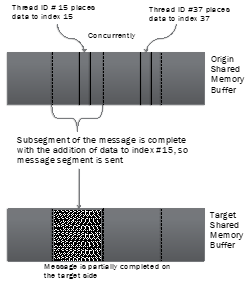
\includegraphics[width=\textwidth]{projects/2.3.1-PMR/2.3.1.17-OMPI-X/partitioned-communications-partial-sends.png}
\end{minipage}
\qquad
\begin{minipage}[c]{0.33\textwidth}
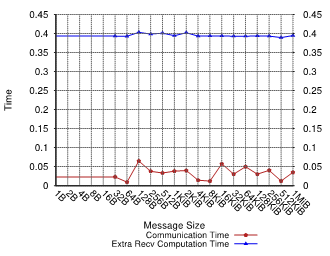
\includegraphics[width=\textwidth]{projects/2.3.1-PMR/2.3.1.17-OMPI-X/partitioned-communications-early-receive.png}
\end{minipage}
\end{figure}

\begin{wrapfigure}{r}{0.40\textwidth}
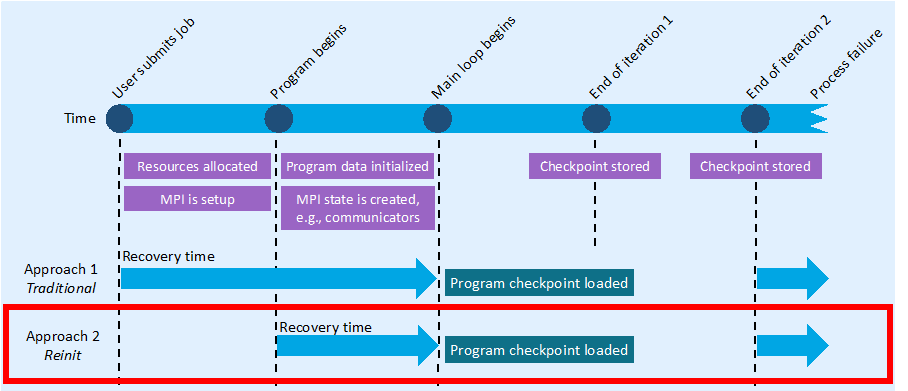
\includegraphics[width=0.40\textwidth]{projects/2.3.1-PMR/2.3.1.17-OMPI-X/reinit.png}
\caption{ReInit reduces application recovery time.}
\label{fig:reinit}
\end{wrapfigure}

\paragraph{Recent Progress}
%% \textit{Describe what you have done recently.  It would be good to
%% have some kind of figure or diagram in this section.}
Through extensive efforts with the MPI Forum community this year, OMPI-X has been successful in 
introducing a number of important exascale-related features into the forthcoming MPI 4.0 standard.
These include sessions, partitioned communications, and a number of error management and recovery features
based on the long-standing User-Level Fault Mitigation (ULFM) concept.  These capabilities have at least
prototype-level implementations available in the Open~MPI library, allowing interested project teams to start
exploring the new capabilities.  We also undertook a cleanup of the Open~MPI code base to improve the quality
of the implementation of some key error handling features. (As in many standards communities, distinctions 
sometimes need to be made between conformance with the standard and providing a ``high-quality'' implementations.)

We are also continuing to drive forward on a number of fronts that did not make the 4.0 version of the standard,
but are still considered important or useful for exascale and the ECP community, particularly in the context of resilience. The ULFM
proposal has been updated to reflect those features that have been incorporated into 4.0, as well as the discussions
within the Forum.  For the complementary Reinit simplified checkpoint/restart proposal (Figure~\ref{fig:reinit}), we have carried out a formal verification on the recovery algorithm. 
This ensures that the protocol, which we plan to propose for a future version of MPI, correctly handles the recovery phase 
of a failure response, including correct propagation of notifications, absence of deadlocks, and proper termination.

We have provided initial implementations of the features above, and more, within the context of the Open~MPI library, to allow
users to explore the new capabilities.  In addition to sessions and partitioned communications, we have expanded the
MPI\_T interface implementation to include events, and implemented a number of new events and performance variables,
demonstrating their use in the context of ECP miniapplications and tools.

Motivated largely by support for the Partitioned Communications proposal and other situations where high network 
concurrency is required, a general user-level threading abstraction has been developed to support both the Qthreads 
and BOLT/Argobots threading libraries within either the Open~MPI or MPICH libraries.  Work begun last year, in 
collaboration with the MPICH and Argobots ECP teams (WBS 2.3.1.07 and 2.3.5.05), has now been integrated into the two MPI implementations.
An important part of the work within Open~MPI involved abstracting the threading layer so that it was not limited to pthreads.

Work on integration with hardware and software environments specifically relevant to the exascale systems continues as well.  On the software
side, we have implemented support for the ALCF's Cobalt resource management system in Open~MPI and PMIx.  This work, which was necessitated by
a major refactoring of Open~MPPI to exclusively use PMIx as its low-level runtime layer, will facilitate support for Aurora, 
which will use a successor to Cobalt.  Combining both software and hardware, we have been working with the SICM ECP project
(WBS 2.3.1.16) to integrate support for complex memory hierarchies into Open~MPI based on SICM's APIs.  This work has now
been demonstrated in several contexts within the Open~MPI library, including the ability to selectively place objects in
either GPU HBM memory or DRAM.  We have also provided a design document for library developers
to work with different memory pools in the context of Open~MPI.  Finally, on the hardware side, we have benefit
working with HPE (Cray) to ensure that the new partitioned communication capability in MPI 4.0 will support GPUs effectively.

In addition to these activities, we continue to support quality assurance of the Open~MPI code base through more and better testing.  The Open~MPI testing infrastructure, 
MTT, continues to be improved for flexibility and capability.  One of this year's noteworthy efforts was the addition of the bueno application test harness to the testing 
system.  The facilitates incorporating third-party test cases (i.e. based on user applications) into the routine testing process without having to commit them to the
Open~MPI testing repository.

\paragraph{Next Steps}
%% \textit{Describe what you are working on next.}
In FY21 and beyond, we plan to continue working across the multiple fronts described above.  We will be in a much better position to work with application teams who can benefit from the new capabilities embodied in MPI 4.0, but who have been reluctant to adopt them until they were officially part of the standard.  We will likewise continue to identify and improve performance and scalability bottlenecks, and to work with HPE (Cray) and the larger community to ensure that their Slingshot network and GPU support are ready for Frontier and Aurora.
